\chapter{Detalles de Implementación y Experimentos}\label{chapter:implementation}
Para poder valorar la viabilidad de la propuesta realizada en este trabajo, es
necesaria la implementación de un prototipo del modelo explicado en el capítulo
anterior.

\section{Herramientas y tecnologías utilizadas}\label{section:implementation:techs}
\subsection{Lenguaje de programación Python}
Python es un lenguaje de programación de propósito general y alto nivel desarrollado por Guido van Rossum en 1991. Su filosofía de diseño enfatiza la legibilidad del código con el uso de sangría significativa. Python se tipifica dinámicamente y tiene incorporado un recolector de basura. Admite múltiples paradigmas de programación, incluida la programación estructurada, orientada a objetos y funcional. La más reciente  versión liberada al momento de realizarse este trabajo es la 3.11 [\cite{python_executive_summary_2022}].

Es altamente empleado para ingeniería y análisis de datos, aprendizaje de máquina
e inteligencia artificial gracias a sus infinidad de bibliotecas como NumPy, Tensorflow, Keras, Pytorch, SciPy, Pandas y Matplotlib, entre otras creadas tanto por el mismo equipo de trabajo de Python como la propia comunidad. Para desarrollo web cuenta con marcos de trabajo (frameworks) como Django. Es altamente utilizado en la educación al ser de fácil aprendizaje y asimilación logrando así reducir la barrera de entrada al mundo de la programación a todo aquel interesado.

 En la actualidad sigue manteniendo el primer puesto de los índices de TIOBE y PYPL ratificando el interés de gran parte de la población y de los empleadores por este lenguaje y las ventajas que ofrece. Grandes organizaciones como Google [\cite{quotes_about_python_2021}], el CERN [\cite{python_the_holy_grail_of_programming_2014}], la NASA [\cite{python_success_stories_2021}], Yahoo [\cite{organizationsusingpython}], Wikipedia, Amazon, Facebook, Instagram [\cite{meta_for_developers_2018}], Spotify, entre otros.
Para este trabajo se utilizó la versión 3.7 para lograr una retro-compatibilidad
alta.


\subsection{Numpy}
Constituye una biblioteca de Python de código abierto, la cual permite generar, tanto vectores como matrices, de grandes dimensiones y operar de manera cómoda y sencilla con ellos [\cite{numpy_2012}].
Consigue esto gracias a que utiliza internamente el lenguaje C para lograr efectuar de forma rápida operaciones muy costosas entre elevadas dimensiones.
En las etapas posteriores a la limpiezas de los datos explicada en el capítulo anterior se utiliza Numpy para el trabajo con los datos.

\subsection{Matplotlib}
Matplotlib es una biblioteca de gráficos creada en 2003 por John D. Hunter para el lenguaje de programación Python y su extensión matemática numérica NumPy. Proporciona una API orientada a objetos para incrustar gráficos en aplicaciones utilizando kits de herramientas GUI de uso general como Tkinter, wxPython, Qt o GTK.
Es una biblioteca completa para crear visualizaciones estáticas, animadas e interactivas. Matplotlib hace que las cosas fáciles, pues sigan siendo fáciles y las difíciles sean posibles, como lo es crear gráficos con calidad de una publicación y hacer figuras interactivas que puedan hacer zoom, desplazarse, actualizar.

%\subsection{Tensorflow, Keras y Addons}
%Tensorflow es una biblioteca de software gratuita y de código abierto para el aprendizaje automático de extremo a extremo y la inteligencia artificial desarrollada por el equipo de Google Brain. Se puede usar en una gran variedad de tareas, pero tiene un enfoque particular en el entrenamiento y la inferencia de redes neuronales profundas. Además brinda interfaces de forma oficial para
%C + +, Haskell, Java, Go, Rust y Python.
%
%Keras es una interfaz de alto nivel de Tensorflow gratuita y altamente productiva para resolver problemas enfocados en el aprendizaje profundo.
%
%Addons es un repositorio de contribuciones que se ajustan a patrones de API bien establecidos, pero implementan nuevas funciones que no están disponibles en el núcleo de TensorFlow. TensorFlow admite de forma nativa una gran cantidad de operadores, capas, métricas, pérdidas y optimizadores.
%
%Para la creación y entrenamiento del modelo de generación de avatares propuesto en la sección \ref{section:proposal:stepbystep} se utilizaron las tecnologías anteriormente mencionadas así como para salvar los pesos del modelo una vez entrenado.

\subsection{Scipy}
SciPy es una biblioteca de Python gratuita y de código abierto que se utiliza para la computación científica y la informática técnica. SciPy contiene módulos para optimización, álgebra lineal, integración, interpolación, funciones especiales, FFT, procesamiento de señales e imágenes, solucionadores de ODE y otras tareas comunes en ciencia e ingeniería. Esta creada encima de la biblioteca Numpy anteriormente mencionada y fue desarrollada por la compañía Enthought en el año 2001.

\subsection{Google Colaboratory}

Google provee un servicio gratuito en el navegador el cual brinda, de manera temporal, recursos computacionales (CPU,TPU,GPU,RAM,HDD) mientras se haga uso activo de los mismos. En dicha plataforma se le permite al usuario escribir y ejecutar codigo Python en un entorno basado en Jupyter Notebook.Siendo así una herramienta ideal para el aprendizaje de máquinas, el análisis de datos y la educación al posibilitar que personas de pocos recursos puedan acceder de forma fácil a herramientas para el aprendizaje de máquina las cuales muchas de ellas ya vienen incluidas en el entorno o son muy  sencillas de instalar en el mismo.
Cabe destacar que además del plan gratuito que incluye CPU de última generación, 13 Gb de RAM y 110 Gb de almacenamiento, nos da la posibilidad de utilizar Google Drive para ampliar el almacenamiento y  varios planes de pago para aumentar la capacidad computacional del entorno.
 
Todo el trabajo fue llevado a cabo utilizando este servicio para dejar de manera accesible todo el flujo de trabajo.

%\subsection{Gensim}
%Gensim es una biblioteca gratuita de Python de código abierto para representar documentos como vectores semánticos, de la manera más eficiente (computacionalmente) y sin dolor (humanamente) posible. Está diseñado para procesar textos digitales crudos y sin estructura ("texto sin formato") utilizando algoritmos de aprendizaje automático no supervisados, entre los que se encuentran implementados Word2Vec [\cite{rehurek_lrec}].

%\subsection{Word2Vec}
%Word2vec es una técnica para el procesamiento del lenguaje natural publicada en 2013. El algoritmo word2vec utiliza un modelo de red neuronal para aprender asociaciones de palabras de un gran corpus de texto. Una vez entrenado, dicho modelo puede detectar palabras sinónimas o sugerir palabras adicionales para una oración parcial. Como su nombre lo indica, word2vec representa cada palabra distinta con una lista particular de números llamada vector. Los vectores se eligen cuidadosamente de modo que capturen las cualidades semánticas y sintácticas de las palabras; como tal, una simple función matemática (similitud de coseno) puede indicar el nivel de similitud semántica entre las palabras representadas por esos vectores.
%Para este trabajo se utilizará el modelo entrenado en 3 mil millones de vocablos en español. Esto nos dota de una gran herramienta que protege la semántica de las palabras ,como se puede evidenciar en la Fig \ref{fig:word2vec}.
%
%\begin{figure}[ht!]
%    \centering
%    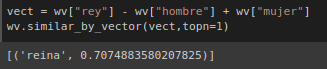
\includegraphics[width=0.6\textwidth]{Graphics/word2vec.png}
%    \caption{Grado de aprendizaje de la semántica de Word2Vec en español}
%    \label{fig:word2vec}
%\end{figure}
%

\subsection{difflib}
Este módulo de Python proporciona clases y funciones para comparar secuencias. Se puede usar, por ejemplo, para comparar archivos y puede producir información sobre diferencias de archivos en varios formatos, incluidos HTML y contexto y diferencias unificadas.

 \subsubsection{clase SequenceMatcher}
 Esta es una clase flexible para comparar pares de secuencias de cualquier tipo, siempre que los elementos de la secuencia se puedan modificar. El algoritmo básico es anterior a un algoritmo publicado a fines de la década de 1980 por Ratcliff y Obershelp con el nombre hiperbólico de ''coincidencia de patrones gestálticos'', y es un poco más elegante. La idea es encontrar la subsecuencia coincidente contigua más larga que no contenga elementos ''basura''; estos elementos ''basura'' son los que no son interesantes en algún sentido, como líneas en blanco o espacios en blanco. (El manejo de basura es una extensión del algoritmo de Ratcliff y Obershelp). Luego, la misma idea se aplica recursivamente a las partes de las secuencias a la izquierda y a la derecha de la subsecuencia coincidente. Esto no produce secuencias de edición mínimas, pero tiende a generar coincidencias que ''parecen correctas'' para las personas.
 \subsubsection{get$\_{}$close$\_{}$matches}
 Método para seleccionar la secuencia más similar a una secuencia dada dentro de un vocabulario.

\subsection{Boto3}
Se utiliza el Kit de desarrollador de software (SDK por sus siglas en inglés) de AWS para Python (Boto3) para crear, configurar y administrar servicios de AWS, como Amazon Elastic Compute Cloud (Amazon EC2) y Amazon Simple Storage Service (Amazon S3). El SDK proporciona una API orientada a objetos, así como acceso de bajo nivel a los servicios de AWS.

Este SDK es empleado para acceder a los datos.

\subsection{pathlib}
Este es un módulo de Python que ofrece clases que representan rutas de sistemas de archivos con semántica apropiada para diferentes sistemas operativos. Las clases de ruta se dividen entre rutas puras, que proporcionan operaciones puramente computacionales sin Entrada/Salida (I/O por sus siglas en inglés), y rutas concretas, que heredan de rutas puras pero también proporcionan operaciones de I/O.

La clase Path de esta biblioteca es ampliamente usada en este trabajo.

\section{Implementación de un prototipo}
El prototipo implementado realiza todos los pasos mencionados en la sección \ref{section:proposal:stepbystep}

Primeramente se realizó todo el trabajo en Google Colaboratory (Colab para abreviar).

\subsection{Extracción de los Datos}
Para la extracción de los datos se utilizó la biblioteca boto3 con acceso al almacenamiento en la nube donde se encontraban los datos.
Para ello se importa el método client de boto3, el cual es instanciado en la url donde se encuentra el conjunto de datos, además de las claves de acceso, las cuales por privacidad del dueño de las mismas se sustituyen por valores de "X". 

\vspace{0.5cm}

\begin{lstlisting}[language=Python, caption={Instanciar cliente s3}, label={code:s3client}]
from boto3 import client

s3_client = client(
    "s3",
    config=Config(
        signature_version="s3v4",
        retries={"max_attempts": 10},
        s3={"addressing_style": "path"},
    ),
    region_name="ams3",
    endpoint_url="https://ams3.digitaloceanspaces.com",
    aws_access_key_id="XXXXXXXXXXXXXXXX",
    aws_secret_access_key="XXXXXXXXXXXXXXXXXXXXXXXXXXXXX",
)
\end{lstlisting}

Una vez obtenido el cliente configurado se descargan los datos del mismo, conociendóse que se encuentran en el bucket "lsc-corpus", los de las señas aisladas, puesto que son los únicos datos con seguridad de la seña que corresponde a cada frase.

\vspace{0.5cm}

\begin{lstlisting}[language=Python, caption={Descargar usando el cliente s3}, label={code:download_s3client}]
from pathlib import Path

root=Path("/content")
bucket="lsc-corpus"    

paginator = s3_client.get_paginator('list_objects_v2')
pages = paginator.paginate(Bucket=bucket)

for page in pages:
    for obj in page['Contents']:
        extension = obj['Key'].split('.')[-1]
        name=obj['Key'].split('.')[0]
        if extension  in ['json']:
		  drivepath=(root/f"tesis-generacion-lsc/{obj['Key']}").resolve()
  		  (drivepath/'..').resolve().mkdir(parents=True,exist_ok=True)
  		  drivepath.touch()
  		  s3_client.download_file(bucket,obj['Key'],str(drivepath))
  
\end{lstlisting}
Aquí se realiza un paginado para poder recorrer de manera adecuada  los elementos del bucket para luego chequear la extensión de los archivos contenidos en cada página.
Se conocen previamente que los datos anotados de los puntos de interés estaban recogidos en archivos con extensión json por cada frase. En la primera parte del código se importa la clase Path de pathlib para trabajar de manera rápida y efectiva con los directorios que se van creando.

\subsection{Limpieza de los datos}
Una vez ya se posean los archivos json referentes a cada frase del corpus se pueden entonces cargarlos para limpiarlos y organizarlos en un dataset mejor estructurado donde estén todas las frases juntas.

En este código utilizamos expresiones regulares para la limpieza de las llaves, ya que incurrían en faltas de ortografía, errores tipográficos y de copiado.
La primera expresión elimina todo lo que esté entre paréntesis en las llaves, puesto que esto no aporta nada a la información semántica de los mismos. Luego se reemplaza todas las ''nn'' por una ''ñ'' 
y se eliminan los dígitos que hayan quedado de manera residual del primer método.Para a modo de cierre de la limpieza de las llaves eliminar todos los guiones entre palabras para que esten de manera individual.
\vspace{0.5cm}

\begin{lstlisting}[language=Python, caption={Cargar los json y limpiar las llaves}, label={code:load_and_clean}]

import numpy as np
import json
import re

root_tesis = (root/f"tesis-generacion-lsc/").resolve()
cendsor_path = "cendsor-corpus/keypoints/"
fps=24

word_poses_dict={}

for dirpath,dirnames,filenames in os.walk(root_tesis/cendsor_path):
  for filename in filenames:
    key,extension=filename.split('.')
	
	###########################
	# Limpieza de las llaves
	###########################
	
    key=re.sub(r"\s*\(.*\)","",key)
    key= key.replace("nn",'ñ')
    key=re.sub(r"\s?\d","",key)
    key = key.replace("-"," ") 
    
	###########################
	
    with open((root_tesis/cendsor_path/filename).resolve(), 'r', encoding='utf-8') as json_list:
      poseframes=np.array(json.load(json_list))
      json_list.close()
		
	  #######################################################
	  # Limpieza y reajuste de los frames de los gestos
	  #######################################################
      filtro = [m!=0.0 for m in  np.mean(poseframes, axis=1)]
      
      poseframes=poseframes[filtro]

      total_frames = poseframes.shape[0]

      n = math.floor(total_frames/fps)

      poseframes= poseframes[::n,:]

      while poseframes.shape[0]>24:
        if poseframes.shape[0]%2:
          poseframes=poseframes[1:,:]
        else:
           poseframes=poseframes[:-1,:]
	  #########################################################
	  
      single_gesture = poseframes.tolist()
      try:
        word_poses_dict[key].append(single_gesture)
      except:
        word_poses_dict[key]=[single_gesture]
        
\end{lstlisting}
En el caso de los gestos existen en el corpus frames en los cuales los modelos no detectaban nada y por tanto estos devolvían (0,0,0) para todos los puntos de interés de ese frame. Por tanto se hace uso de la biblioteca json para cargar el archivo y de la biblioteca numpy para realizar la limpieza de una manera más cómoda y rápida.
Luego de obtener la máscara (filtro) con la información de los frames vacíos, simplemente se indexa en el arreglo numpy guardando su resultado como si fuera ahora el arreglo original.
Pero proseguía un problema más, el tamaño de los frames no era parejo. Algunos archivos tenían más frames que otros, por lo tanto se decidió llevarlos todos a 24 frames utilizando la función floor de la biblioteca math para obtener un valor que al dividir por la cantidad de frames no diera superior y fuera entero.
Posteriormente, como no van a quedar exactamente de tamaño 24, sino mayor, se va reduciendo en 1 la cantidad de frames por los extremos hasta llegar a la cantidad deseada.

Como información adicional se guarda el diccionario tanto en la nube como en local para su mejor aprovechamiento y eliminarnos pasos extras a la hora de probar el modelo.

%\subsection{Cargando el embedding de palabra}
%Primeramente se debe descargar el archivo de los KeyedVectors el cual pesa alrededor de los 3Gb, razón por la cual se ha estado desarrollando todo este flujo de trabajo directamente en Colab puesto que es un gran modelo para capturar significado semántico dado lo limitado del corpus en ese sentido.
%\vspace{0.5cm}
%
%\begin{lstlisting}[language=Bash, caption={Descargar datos del modelo KeyedVectors de su sitio web}] 
%  
%  $ wget "https://zenodo.org/record/1410403/files/keyed_vectors.zip" 
%  $ unzip keyed_vectors.zip
%  
%\end{lstlisting}
%
%Luego de descargado y descomprimido se puede entonces cargar el modelo.
%
%\begin{lstlisting}[language=Python, caption={Cargar modelo de KeyedVectors}]
%  from gensim.models import KeyedVectors
%  wv = KeyedVectors.load('complete.kv', mmap='r')
%\end{lstlisting}
%Como se aprecia, KeyedVectors es un modelo perteneciente a la biblioteca gensim, el cual es uno de los elementos que componen a Word2Vec y justamente el único que necesitamos para nuestro propósito de  capturar la semántica de las frases. Cargar completamente el modelo Word2Vec exige mucha memoria RAM puesto que es un modelo de más de 7 Gb en su completitud y es esa la razón por la que se escoge solamente el diccionario de los vectores claves (KeyedVectors).
%
%.El archivo complete.kv es el resultado de descomprimir el modelo descargado.
\subsection{Encontrando similitud de palabras}
Como se plantea en la propuesta primeramente se debe asegurar de que se logre encontrar una palabra dentro del vocabulario de nuestro embedding, por eso se declara el siguiente método a continuación.

\begin{lstlisting}[language=Python, caption={Método para encontrar palabras similares en un vocabulario}]
  def find_similar(word, vocab):
  	import difflib
  	best_match=difflib.get_close_matches(word,vocab)
  	if len(best_match) != 0:
    	score = difflib.SequenceMatcher(None,word,best_match[0]).ratio()
    	return best_match[0],score
    else:
    	return None
    	
\end{lstlisting}
En este método se utiliza el método get$\_{}$close$\_{}$matches para encontrar la palabra más parecida sintácticamente a la proporcionada, en el vocabulario dado.
Luego si encuentra que existe alguna palabra que sea similar, pues se instancia una clase SequenceMatcher para hallar que tan similares son. Por supuesto este ultimo paso solo es necesario en caso de necesitarse cuantificar la similitud.

%\subsection{Extrayendo la matriz de cada frase}
%El siguiente método genera una matriz de $num\_{}vecs$ x $vec\_{}dim$ que es la dimensión de los vectores. 
%Primero se crea un diccionario de palabras mal escritas (posible en este escenario dado que solo se cuentan con poco más de 1050 vocablos) y además para no arrastrar el error semántico de unos datos erróneos se escogen palabras de igual significado semántico.
%
%Luego se crea un arreglo numpy de ceros con las dimensiones específicadas para posteriormente conformarlo con los vectores de cada palabra de la frase de 5 vocablos en el caso del corpus utilizado.
%
%\begin{lstlisting}[language=Python, caption={Obtener el vector dada una palabra}]
%  def get_vector(key,word_vectors,num_vecs=5):
%  wrong_words={'antonimo': 'antónimo',
%              'audiologia':'audiología',
%              'barsura':'basura',
%              'defectologia':'defectología',
%              'empanizar':'empanar',
%              'insipido': 'insípido',
%              'investar':'inventar',
%              'lexicologia': 'lexicología',
%              'ostion':'ostra',
%              'panciencia':'paciencia',
%              'policlinica': 'policlínica',
%              'querologia':'querología',
%              'rehablilitacion':'rehabilitación',
%              'sacapunta':'sacapuntas',
%              'señacionario':'diccionario',
%              'señario':'libro', 
%              'zapia':'compartición'}
%  vector=np.zeros((num_vecs,word_vectors.vector_size))
%  
%  for i,word in enumerate(key.split(" ")):
%    if word in word_vectors.vocab.keys():
%
%      wordvec = word_vectors[word]
%    else:
%      word=wrong_words[word]
%      nword, similarity = find_similar(word,word_vectors.vocab.keys())
%      print(key,"Not Founded")
%      print(nword,similarity)
%
%      wordvec = word_vectors[nword]
%    vector[i:]=wordvec
%  return vector
%\end{lstlisting}
%Luego de creado el arreglo de numpy, se verifica que la palabra esté en el vocabulario del embedding antes de indexar la palabra en busca de su vector. En caso de no existir la palabra pues se utiliza el método descrito en la subsección anterior para hallar un vocablo sintácticamente similar que si pertenezca al vocabulario del embedding.
%
%Finalmente, después de rellenado el arreglo de numpy, este es retornado.

%\subsection{Creando los conjuntos}
%
%En este código creamos y llenamos los conjuntos $X$ e $y$ para su ulterior uso en el modelo. $num\_{}vecs$ es escogido como el mayor número de palabras de todo el conjunto de datos, el cual en exploraciones a los datos fue revelado que es 5.
%
%\begin{lstlisting}[language=Python, caption={Crear los conjuntos X e y}]
%  
%X=[]
%y=[]
%
%num_vecs=max([len(key.split(" ")) for key in dataset.keys()])
%
%for key,gestures in dataset.items():
%  vector=get_vector(key,word_vectors,num_vecs)
%  X.append(vector)
%  y.append(np.array(gestures[0]).reshape((fps,sum([dim[0] for dim in dims]),dims[0][1]))) 
%\end{lstlisting}
%Para evitar el problema de que a cada frase le correspondieran varias señas, con alta probabilidad de que fueran distintas, se optó por solamente escoger la primera de las señas como representativa de las demás.

\subsection{Métodos para la animación}
Primero instanciamos los valores necesarios para animar correctamente un conjunto de puntos con estructura igual a la de los datos .

\begin{lstlisting}[language=Python, caption={Instanciar datos necesarios para animar }]
body_dim = 25*3
left_dim = 21*3
right_dim = 21*3

dims=[(25,3),(21,3),(21,3)]

bodyjoints=[[1,7],[4,8],[9,10],[11,12],[11,13],
[12,14],[11,23],[12,24],[23,24],[13,15],[14,16]]
leftjoints=[[0,1],[1,2],[2,3],[3,4],
            [0,5],[5,6],[6,7],[7,8],
            [5,9],[9,10],[10,11],[11,12],
            [9,13],[13,14],[14,15],[15,16],
            [13,17],[17,18],[18,19],[19,20],[0,17]]
rightjoints=leftjoints

fullbodyjoints=[bodyjoints,leftjoints,rightjoints]

parts_names=["body","left","right"]
\end{lstlisting}

Utilizamos el siguiente método en caso de que los puntos no vengan en formato (24,67,3) y simplemente vengan en formato (24,201)

\begin{lstlisting}[language=Python, caption={Extraer las partes en 3d }]
def extract_3d_shape(array,dims):
      init=0
      ending=0
      parts=[]
      for dim in dims:
        ending+=dim[0]*dim[1]
        parts.append(array[:,init:ending].reshape((array.shape[0],dim[0],dim[1])))
        init+=dim[0]*dim[1]

      single_gesture={parts_names[i]:parts[i] for i in range(len(dims))}

      return single_gesture
\end{lstlisting}

Utilizamos la lista con las dimensiones para de poder, en caso de ser necesario, incluir graficaciones de otras partes del cuerpo que fueron excluidas.

El siguiente método contituye la base de todos los métodos para las animaciones de este trabajo.
Se utilizan varias clases y métodos de la biblioteca matplotlib para realizar la animación.

FuncAnimation recibe la figura en la que trabajar,la función de actualización, que es la encargada de la transición entre frames, y por último la cantidad de frames a animar.

\begin{lstlisting}[language=Python, caption={Método base para animar }]
import matplotlib.pyplot as plt
from matplotlib.animation import FuncAnimation
from matplotlib import rc
import matplotlib.cm as cm

def transform_data(Data,i):
    from scipy.spatial.transform import Rotation as R

    r = R.from_rotvec(np.pi/2 * np.array([0,0,1]))

    X=np.array(Data[i,:,0])
    Y=np.array(-Data[i,:,1])
    Z=np.array(Data[i,:,2])
    meanpoint=(X[X!=0].mean(),Y[Y!=0].mean(),Z[Z!=0].mean())

    D = np.array([x if x!=(0.0,0.0,0.0) 
                    else meanpoint
              for x in zip(X, Y, Z) ])
    D = r.apply(D)
    return D

def animate(
			Data,
			frames=None,
			figsize=(7.0,3.5),
			elev=None,
			angle=None,
			dims=dims,
			text=False,
			joints=False):
			
  rc('animation',html='jshtml')
  fig_size_x,fig_size_y=figsize

  plt.rcParams["figure.figsize"]= [fig_size_x,fig_size_y]
  plt.rcParams['figure.autolayout']= True

  fig = plt.figure()
  ax = fig.add_subplot(projection='3d')
  colors=['b','y','r','k']
  
  def update(i):
    ax.clear()

	D = transform_data(Data,i)	
	
    s=0
    e=0
    for j, dim in enumerate(dims):
      dim = dim[0]
      e+=dim

      x=D[s:e,0]
      y=D[s:e,1]
      z=D[s:e,2]

      # print((x.mean(),y.mean(),z.mean()) != meanpoint )
      if (x.mean(),y.mean(),z.mean()) != meanpoint:
        # print(x.mean(),y.mean(),z.mean())
        ax.plot(D[s:e,0],D[s:e,1],D[s:e,2],f'{colors[j]}.')
      if text:
        for p in range(s,e):
          ax.text3D(D[p,0],D[p,1],D[p,2],str(p))
      if joints:
        for h,k in fullbodyjoints[j]:
          ax.plot([D[s+h,0],D[s+k,0]],[D[s+h,1],D[s+k,1]],[D[s+h,2],D[s+k,2]],f'{colors[j]}')
      s+=dim

    ax.set_axis_off()
    if elev and angle:
      ax.view_init(elev,angle) 

    
    return ax

  if frames is None:
    frames=24
  return FuncAnimation(fig,update,frames=frames,repeat=True)
\end{lstlisting}

Se utiliza la clase Rotation del módulo transform de scipy para rotar de manera efectiva la figura para que sea visualmente atractiva la animación desde una vista frontal. Al igual que si existen muchos puntos espaciales en el (0,0,0) se halla la media de los puntos distintos del cero del espacio para no distorsionar el graficado de la animación, esto ocurre por fallos del método que creó el corpus inicialemente al no detectar alguna región del cuerpo, es decir ya los datos con los que se cuentan vienen dados con cierto grado de error.
Luego, para que sea visualmente llamativo, se utilizan las dimensiones de las distintas partes del cuerpo para graficar de un color diferente cada una de las partes y se utilizan las uniones declaradas inicialmente. 

En caso de ser necesario puede agregarse el texto del número correspondiente al punto para mejor visualización.

También se incorpora la posibilidad de modificar las dimensiones de la figura, así como el angl¡ulo de azimut y de elevación correspondiente.


En cuanto al último método, este solo representa una composición de los métodos anteriores con una organización intermedia de los arreglos correspondientes a cada parte en caso de que la entrada no tenga la estructura idónea para la graficación.

\begin{lstlisting}[language=Python, caption={Graficar la animación }]
  
def plotanimation(result):
	if result.shape[2]==201:
  		dict_parts=extract_3d_shape(result[0],dims)
      
  		body_frames = dict_parts["body"]
  		left_frames = dict_parts["left"]
  		right_frames = dict_parts["right"]

  		result = np.hstack((body_frames,left_frames,right_frames))
  		

  a=animate(result,result.shape[0],(12,10),90,1,dims,text=False,joints=True)
  
  return a
\end{lstlisting}

%\section{Entrenamiento}
%El modelo presentado, como se mencionó en capítulos anteriores, necesita ser debidamente entrenado. Dado que el dominio e imagen del conjunto disponible para el entrenamiento es alarmantemente corto en comparación con los vocablos utilizados comúnmente en el día a día por una persona promedio. Hablamos de que alrededor de 20 mil vocablos son empleados a diario en una jornada normal, mientras que el corpus brindado por el CENDSOR solo cuenta con poco más de 1050 vocablos(con algunos teniendo más de 1 respresentación visual diferente)
%
%Con estas condiciones del corpus, el enfoque adoptado para el entrenamiento es el de generar sobreadecuación (overfitting) sobre los únicos vocablos conocidos para que así al componerse con el uso del embedding de palabra puedan encontrarse similaridades semánticas entre una palabra desconocida y una del vocabulario disponible.
%subsection{Definición del modelo}
%
%Como se explicó en la propuesta, el enfoque adoptado para este modelo es el de utilizar redes neuronales recurrentes, más específicamente LSTM multicapas con capas deconvolucionales para ampliar las dimensiones.
%\begin{lstlisting}[language=Python, caption={Diseño del modelo}]
%
%from tensorflow.keras.layers import InputLayer, LSTM , Conv1DTranspose, Reshape
%from tensorflow.keras.models import Sequential
%from tensorflow_addons.metrics.r_square import RSquare
%
%def get_model(X, y):
%    model = Sequential()
%    model.add(InputLayer(X.shape[1:]))
%    model.add(LSTM(128, return_sequences=True, activation="relu"))
%    model.add(LSTM(256, return_sequences=True, activation="relu"))
%    model.add(Conv1DTranspose(filters=100,kernel_size=10))
%    model.add(LSTM(128, return_sequences=True, activation="relu"))
%    model.add(Conv1DTranspose(filters=150,kernel_size=11))
%    model.add(LSTM(201,return_sequences=True))
%    model.add(Reshape(y.shape[1:]))
%    loss = "mae"
%    metrics = RSquare()
%    model.compile(optimizer='Adam', loss=loss, metrics=metrics)
%    return model
%\end{lstlisting}
%
%Las cantidad de unidades fueron escogidas basándonos en la unidades que reportaron beneficios para el trabajo precedente a este [\cite{leynier-lsc-2021}].
%Para la función de pérdida fue seleccionado el Error Medio Absoluto(MAE por sus siglas en inglés) puesto que compara efectivamente la diferencia de posición espacial dados los datos con que se cuentan.
%Además se usa el R Cuadrado como métrica de puntuación para poder entrenar de manera efectiva.
%
%
%Las opciones basadas en transformadores requerían de cantidades de datos superiores a las que se contaban así que se tomó solo en cuenta los estudios referentes a las Redes neuronales recurrentes LSTM.
%
%
%Se utilizó un método supervisado de entrenamiento usando un enfoque regresivo dada la no existencia de categorías calaramente definidas en el espacio de todas las posibles señas.
%\begin{lstlisting}[language=Python, caption={Graficar la animación }]
%
%
%from tensorflow.keras.callbacks import EarlyStopping, ModelCheckpoint
%from sklearn.model_selection import KFold,cross_val_score
%
%X,y=(np.array(X),np.array(y))
%X_train,X_test,y_train,y_test = train_test_split(X,y,test_size=0.3,random_state=42)
%
%checkpoint_path= (droot_tesis/"generacion-lsc_0001.ckpt").resolve()
%
%num_folds=5
%batch_size=32
%epochs=1000
%
%kfold = KFold(n_splits=num_folds, shuffle=True)
%
%# K-fold Cross Validation model evaluation
%acc_per_fold=[]
%loss_per_fold=[]
%fold_no = 1
%for train, val in kfold.split(X, y):
%
%  model = get_model(X, y)
%  if checkpoint_path.exists():
%    model.load_weights(checkpoint_path)
%
%  ckpt_callback= ModelCheckpoint(
%      filepath=str(checkpoint_path).format(epoch=0),
%      save_weights_only=True,
%      verbose=1,
%      save_freq=5*batch_size)
%  
%  callback = EarlyStopping(
%      monitor= "loss",
%      patience=10)
%  
%  print(model.summary())
%  # Generate a print
%  print('--------------------')
%  print(f'Training for fold {fold_no} ...')
%
%  # Fit data to model
%  history = model.fit(
%      X[train],
%       y[train],
%       batch_size=batch_size,
%       epochs=epochs,
%       callbacks=[callback,ckpt_callback])
%
%  # Generate generalization metrics
%  scores = model.evaluate(X[val], y[val],)
%  print(f'Score for fold {fold_no}: {model.metrics_names[0]} of {scores[0]}; {model.metrics_names[1]} of {scores[1]*100}%')
%  acc_per_fold.append(scores[1] * 100)
%  loss_per_fold.append(scores[0])
%
%  # Increase fold number
%  fold_no = fold_no + 1
%
%\end{lstlisting}
%
%Se utiliza un entrenamiento con Kfold para iterar por conjuntos de datos separados de forma aleatoria y así lograr evaluar para todos los valores además de 1000 epochs.
%Se utilizan callbacks de parada temprana para en caso de que los valores de las funciones de puntuación y de pérdida no varían mucho luego de un cierto tiempo y además se usa un callback para salvar los pesos del modelo durante el entrenamiento en caso de colapso del servicio de Colab o de fallos eléctricos. 
%Dicha salva de los pesos del modelo es retomada en cada iteración del método Kfold para garantizar que se haga overfitting sobre los datos.
%
%Podrá parecer extraño que se quiera sobreadecuar el modelo al conjunto de datos pero no es la primera vez que se hace esto sobre el vocabulario disponible de cierta tarea o problema, como se hizo en el caso de GPT3, el cual sobreadecúa los datos de todo internet logrando así dominar el vocabulario dado.

\subsection{Experimentos}
%Como desenlace del entrenamiento del modelo se logró evidenciar buenos resultados dada la simpleza del método presentado, las limitantes y problemáticas del conjunto de datos.
%
%\begin{figure}[ht!]
%    \centering
%    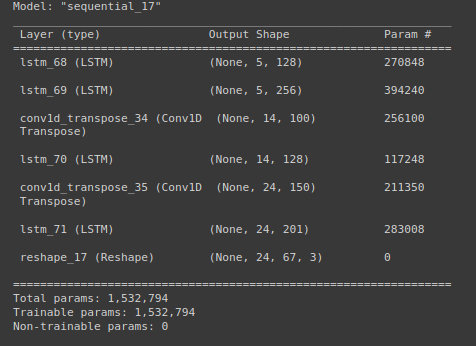
\includegraphics[width=0.8\textwidth]{Graphics/resumen_modelo.png}
%    \caption{Resumen de las capas y parametros del modelo}
%    \label{fig:resumen_modelo}
%\end{figure}
%
%Durante el entrenamiento se utilizaron las métricas Error Promedio Absoluto (MAE por sus siglas en inglés) como función de pérdida y R Cuadrado (R Squared) como función de puntuación dado que este es un problema de regresión.
%
%
%\begin{figure}[ht!]
%    \centering
%    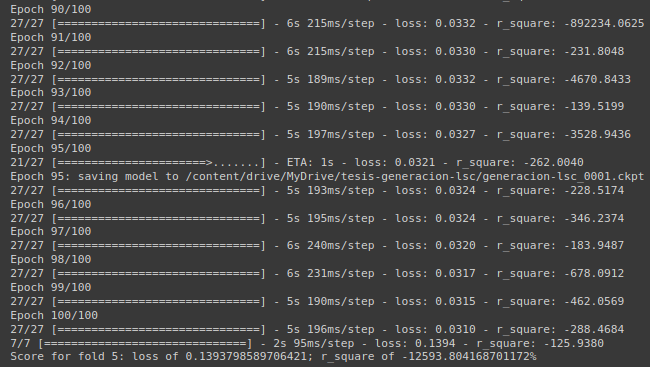
\includegraphics[width=0.8\textwidth]{Graphics/metricas_last_epochs.png}
%    \caption{Resultado de las métricas de los últimos epochs del modelo durante el entrenamiento}
%    \label{fig:metricas_last_epochs}
%\end{figure}
%
%Aquí se puede presenciar una comparativa de los resultados obtenidos para la primera frases del conjunto de datos.
%
%\begin{figure}[ht!]
%    \centering
%    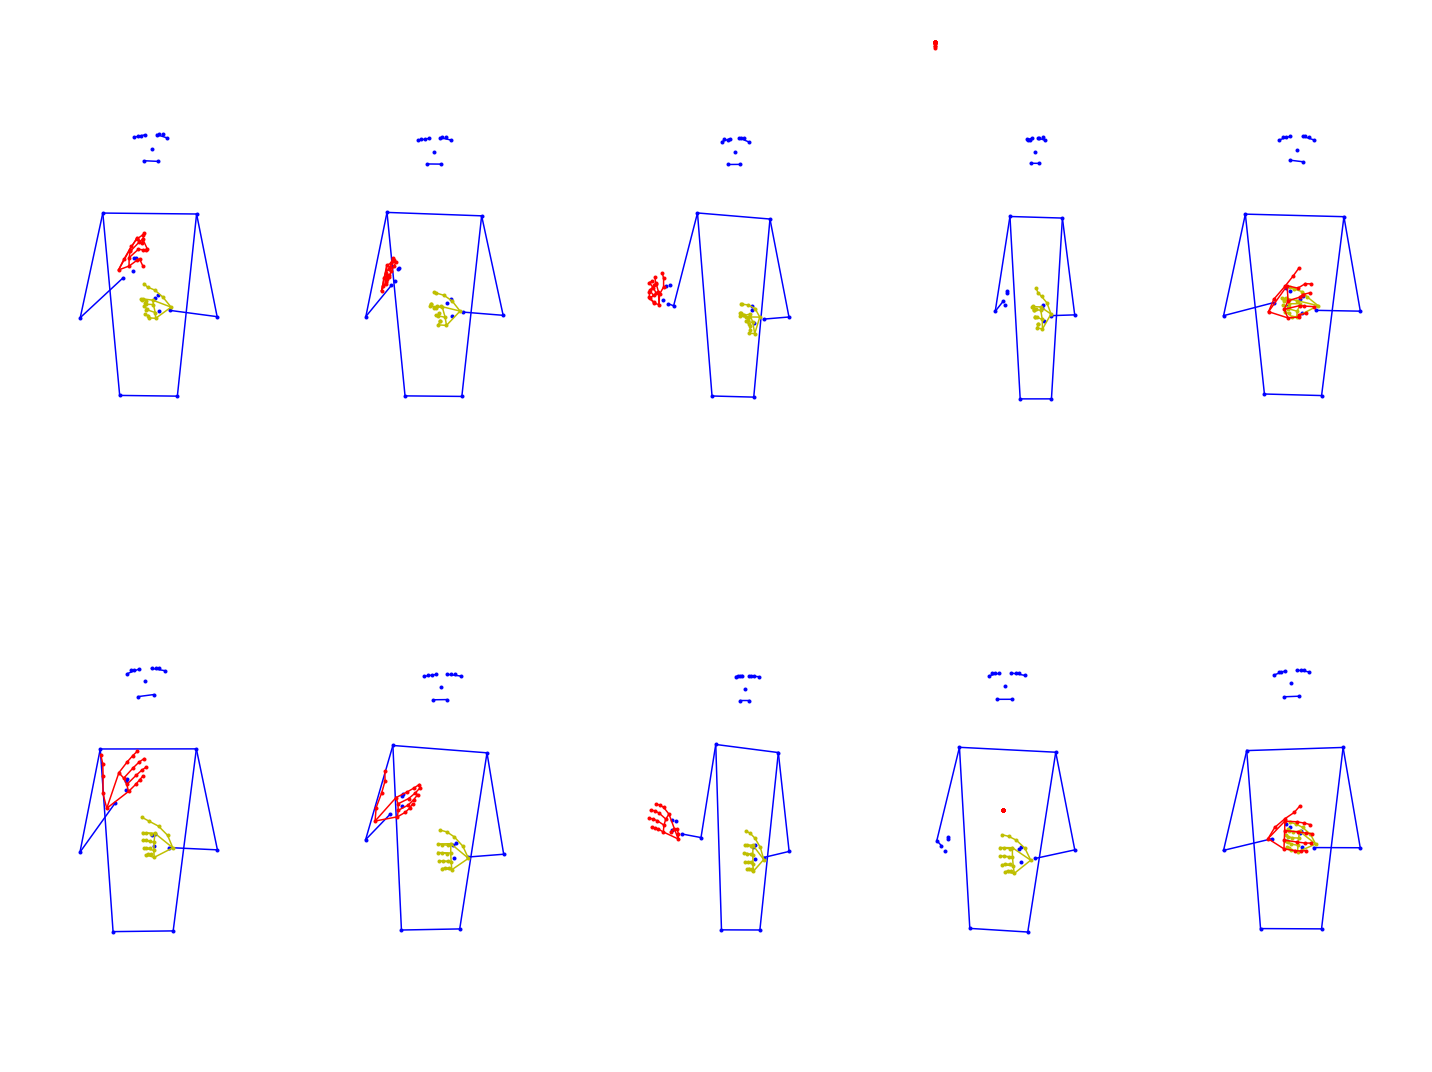
\includegraphics[width=0.8\textwidth]{Graphics/abandonar_comparison.png}
%    \caption{Comparativa de la frase ''abandonar'' . Fila superior los valores predichos. Fila inferior los valores reales}
%    \label{fig:abandonar_comparison}
%\end{figure}
%
%\begin{figure}[ht!]
%    \centering
%    \includegraphics[width=0.8\textwidth]{Graphics/por_la_mañana_comparison.png}
%    \caption{Comparativa de la frase ''por la mañana'' . Fila superior los valores predichos. Fila inferior los valores reales}
%    \label{fig:mannana_comparison}
%\end{figure}

\subsection{Discusión}
%Visualmente se obtuvieron buenos resultados, pero sin una medida específica salvo la percepción del autor.
%Muchos de los puntos referentes a los dedos no se detectaron como se correspondía y no se tuvo una métrica que describiera bien la puntuación del modelo de regresión.
% Esto se debe en gran parte a que los datos con que se contaban presentaban errores y, al ser pocos, se transmitían de manera fácil al modelo durante el entrenamiento, a pesar de emplear la sobreadecuación del mismo al corpus brindado.
%
%A pesar de ello se obtuvieron resultados bastante aceptables y una puntuación del R Cuadrado bastante cercana al máximo posible que es 1.